\chapter[Avaliação da Ferramenta]{Avaliação da Ferramenta}
\label{cap:cap4}

Nesse capítulo, são apresentadas a metodologia utilizada para avaliação de usabilidade da ferramenta e-TAPE, assim como a a análise dos resultados obtidos.

% 1a seção do capítulo 4
\section{Cenário da Avaliação}
\label{sec:cenario}
O objetivo desta avaliação foi analisar a usabilidade da e-TAPE através de um experimento no qual potenciais usuários pudessem utilizar a ferramenta. A avaliação foi dividida em três etapas: na primeira, foi realizada a identificação do perfil dos participantes e apresentação do experimento, na segunda etapa, os participantes utilizaram a e-TAPE executando tarefas que foram pré-determinadas, por último, foi realizada avaliação de usabilidade da ferramenta.

\par
Na primeira etapa, os participantes foram informados quanto ao objetivo do experimento e orientados sobre os procedimentos a serem seguidos de maneira que os usuários tivessem um entendimento da tarefa a ser desenvolvida. 
A coleta de dados sobre o perfil foi realizada através de um questionário, descrito na tabela \ref{tab:questionario}. 

\begin{table}[!ht]
    \centering
    \caption{Dados coletados sobre o perfil dos participantes}
    \label{tab:questionario}
    \begin{tabular}{l*{2}{>{\raggedright\arraybackslash}p{0.2\linewidth}}}
    \toprule
        Pergunta        \\
    \midrule
        Qual seu sexo? \\
        Qual sua idade?\\
        Qual seu grau de escolaridade?\\
        Você conhece o conceito de participação eletrônica?\\
        Se respondeu sim na pergunta anterior,\\ por onde conheceu o conceito de participação eletrônica?\\
        Você costuma discutir questões sociais na internet?\\
        Se respondeu sim na pergunta anterior,\\ costuma discutir com: \\
        a) amigos, colegas ou conhecidos b) desconhecidos c) Ambos \\ 
        Caso você discuta questões sociais na internet, qual(is) ferramentas utiliza? \\
        Você sabe o que é uma Taxonomia?\\
    \bottomrule
    \end{tabular}
\end{table}

\par
Após a primeira etapa, foi disponibilizada uma máquina com acesso à internet para que os participantes pudessem acessar a e-TAPE. Foi dado cinco minutos para que cada usuário pudesse se informar sobre a TAPE lendo as definições dos grupos, classes e subclasses,
disponíveis na primeira página da aplicação. 
Após os cinco minutos, foi entregue a cada usuário duas descrições textuais sobre ferramentas de participação eletrônica. Essas descrições foram elaboradas com o auxílio dos pesquisadores envolvidos na construção da TAPE que são especialistas em participação eletrônica. 
A partir dessas descrições, cada usuário deveria classificar a ferramenta descrita usando a e-TAPE de acordo com o que achasse mais adequado.
Essa abordagem foi adotada para que fosse possível a comparação entre a classificação de uma ferramenta de participação feita por um especialista em comparação com a classificação por usuários leigos. O tempo gasto para leitura das descrições textuais e classificação das ferramentas foi cronometrado e registrado.
As descrições de ferramentas apresentadas aos participantes estão disponíveis no Apêndice \ref{apendice:c}.

\par
Na terceira etapa, após finalizada a interação do participante com a ferramenta, o objetivo foi avaliar a usabilidade da e-TAPE.
Para essa avaliação, foi utilizado o questionário \acrfull{sus}, desenvolvido por \citeonline{brooke1996sus} e composto por 10 questões que foram definidas após a aplicação de um questionário sobre dois sistemas diferentes com 50 itens em potencial. Desses 50 itens, foram selecionados os 5 com os maiores valores de concordância e os outros 5 com maiores valores de discordância. Os 10 itens selecionados
foram postos alternadamente, com o objetivo de evitar respostas automáticas, obrigando o respondente a se esforçar para pensar se concorda ou discorda com cada item. 

\par

Cada questão é associada a uma escala \textit{likert} de 5 pontos, sendo o valor 1 atribuído ao discordo totalmente e o 5 atribuído ao concordo totalmente.
A figura \ref{fig:exemplo-pergunta} exemplifica a escala utilizada.

\begin{figure}[!ht]
    \centering
    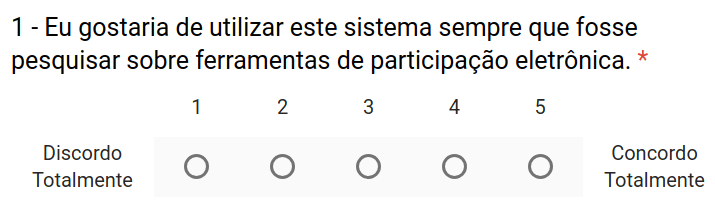
\includegraphics[scale=0.4]{./figuras/exemplo_pergunta.png}
    \caption{Exemplo de um item \textit{Likert}}
    \label{fig:exemplo-pergunta}
\end{figure}

\par
 As 10 questões são obrigatórias, caso o participante não saiba como responder a algum item em especial, deve-se solicitar que responda-o com o valor três, ou seja, o ponto central da escala. A coleta das respostas 
deve ser feita imediatamente ao término da leitura de cada item, evitando o prolongamento do tempo de resposta que, de acordo com os autores, pode influenciar de alguma maneira \cite{brooke1996sus}.

\par

O questionário \acrshort{sus} permite o cálculo de um indicador para a usabilidade geral do sistema avaliado, denominado \textit{Score SUS}, que varia entre 0 e 100. 
\citeonline{brooke1996sus} definiram o cálculo do \textit{Score SUS} da seguinte forma:
para os itens 1, 3, 5, 7 e 9, será o valor assinalado pelo respondente menos 1; para os itens 2, 4, 6, 8 e 10, será 5 menos o valor assinalado. Após isso, a soma dos valores 
encontrados é multiplicada por 2,5, obtendo-se o \textit{Score SUS} para o sistema avaliado. \citeonline{sauro2015supr} chega a conclusão, após um estudo feito com 500 aplicações, 
que um \textit{Score SUS} maior ou igual 68.0 deve ser considerado acima da média em relação à usabilidade.

\par
O questionário proposto no trabalho original está descrito no Anexo \ref{anexo:questionario} e foi adaptado ao contexto de utilização da e-TAPE de maneira que as especificidades desse domínio fossem consideradas na avaliação. 
O questionário utilizado está descrito pela Tabela \ref{tab:questionario3}.

\begin{table}[!ht]
    \centering
    \caption{Questionário SUS adaptado para avaliação da e-TAPE}
    \label{tab:questionario3}
    \begin{tabular}{l*{2}{>{\raggedright\arraybackslash}p{0.66\linewidth}}}
    \toprule
    Nº & Questão        \\
    \midrule
    1 & Eu gostaria de utilizar este sistema sempre que fosse pesquisar sobre ferramentas de participação eletrônica.\\
    2 & Eu achei a aplicação desnecessariamente complexa. \\
    3 & Eu achei a aplicação fácil de usar.\\
    4 & Eu acho que precisaria de apoio de um suporte técnico para ser possível interagir com essa aplicação.\\
    5 & Eu achei que as diversas funções nesta aplicação foram bem integradas. \\
    6 & Eu achei que houve muita inconsistência ou erros nesta aplicação. \\
    7 & Eu imaginaria que a maioria das pessoas, interessadas em ferramentas de participação eletrônica, aprenderia a usar essa aplicação rapidamente. \\
    8 & Eu achei a aplicação muito complicada. \\
    9 & Eu me senti muito confiante quanto às interações com essa aplicação. \\
    10 & Eu precisei aprender muitas coisas sobre ferramentas de participação eletrônica para que eu pudesse fazer uso da aplicação.\\
    \bottomrule
    \end{tabular}
\end{table}


\par
\citeonline{boucinha2013avaliaccao} afirmam que as questões do \acrshort{sus} podem ser associadas aos componentes de qualidade descritos por \citeonline{nielsen199510},
da seguinte forma:

\begin{table}[!ht]
    \centering
    \caption{Componentes de qualidade de \citeonline{nielsen199510} x Questões \acrshort{sus}}
    \label{tab:componentesQualidadePorQuestao}
    \begin{tabular}{l*{2}{>{\raggedright\arraybackslash}p{0.2\linewidth}}}
    \toprule
        Componente de Qualidade & Questão(ões)        \\
    \midrule
        Facilidade de aprendizagem & 3, 4, 7 e 10 \\
        Eficiência & 5, 6 e 8 \\
        Facilidade de memorização & 2 \\
        Minimização dos erros & 6 \\
        Satisfação & 1, 4 e 9\\
    \bottomrule
    \end{tabular}
\end{table}

\par 
De acordo com os autores, para avaliar cada componente de qualidade, deve-se fazer a média dos valores encontrados no cálculo do \textit{Score SUS} para o grupo de perguntas 
em questão \cite{nielsen199510}. Os resultados encontrados foram analisados e estão descritos na Seção \ref{sec:resultados}. 

\section{Resultados}
\label{sec:resultados}

Seguindo a metodologia utilizada, foi solicitado aos participantes que respondessem ao questionário. Participaram 12 voluntários no experimento, sendo 75\% do sexo masculino e 25\% do sexo feminino, como apresentado no gráfico da Figura \ref{fig:grafico-sexo}. Além disso, 
é possível observar, pela Figura \ref{fig:grafico-idade}, que a maioria dos participantes tem entre 21 e 25 anos de idade e 
estão com a graduação atualmente em curso, como representado na Figura \ref{fig:grafico-grau}.

\begin{figure}[!ht]
    \centering
    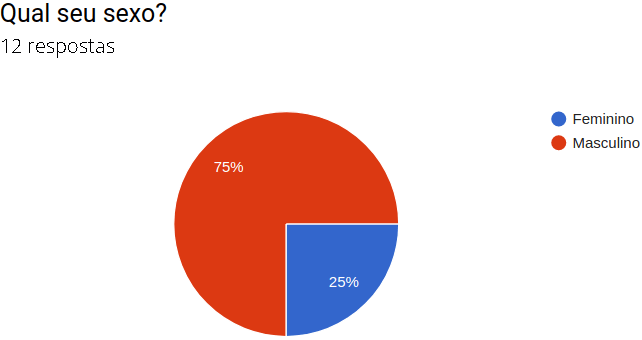
\includegraphics[scale=0.4]{./figuras/sexo.png}
    \caption{Sexo dos participantes}
    \label{fig:grafico-sexo}
\end{figure}

\begin{figure}[!ht]
    \centering
    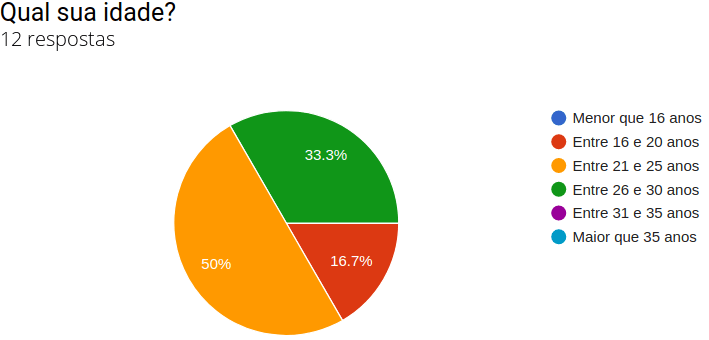
\includegraphics[scale=0.4]{./figuras/idade.png}
    \caption{Idade dos participantes}
    \label{fig:grafico-idade}
\end{figure}

\begin{figure}[!ht]
    \centering
    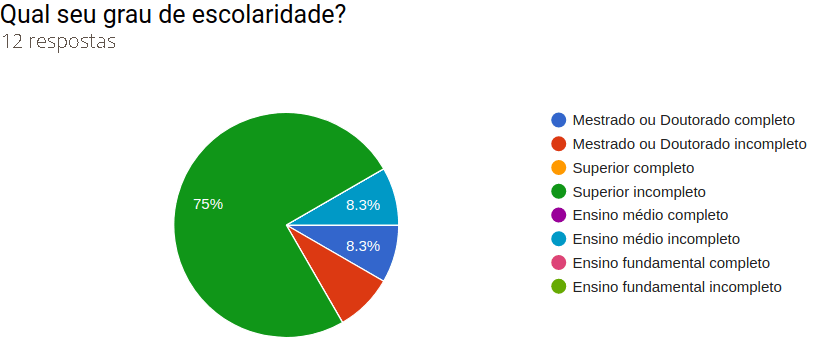
\includegraphics[scale=0.4]{./figuras/grau_escolaridade.png}
    \caption{Grau de escolaridade dos participantes}
    \label{fig:grafico-grau}
\end{figure}

\par
Pôde-se perceber que a maioria dos participantes, 91,7\%, não conhecia o conceito de participação eletrônica, resultado descrito na Figura \ref{fig:grafico-participacao}.

\begin{figure}[!ht]
    \centering
    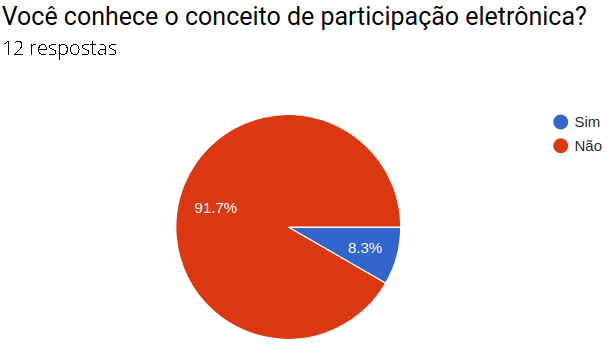
\includegraphics[scale=0.4]{./figuras/conhece_participacao_eletronica.png}
    \caption{Conhecimento sobre o conceito de participação eletrônica dos participantes}
    \label{fig:grafico-participacao}
\end{figure}

\par
Contudo, 58,3\% dos participantes responderam que costumam discutir questões sociais na internet (Figura \ref{fig:grafico-discu-alvo}). 
Desses, 80,0\% disseram que  discutem com amigos, colegas ou conhecidos, 20,0\%  responderam que discutem com ambos, ou seja, amigos, colegas ou conhecidos e desconhecidos. Esse resultado está representado no gráfico da figura \ref{fig:grafico-discu-alvo}. Quando perguntados sobre quais ferramentas de participação 
eletrônica eles utilizam para discutir esse tipo de questão, 100\% das respostas foram redes sociais. 

\begin{figure}[!ht]
    \centering
    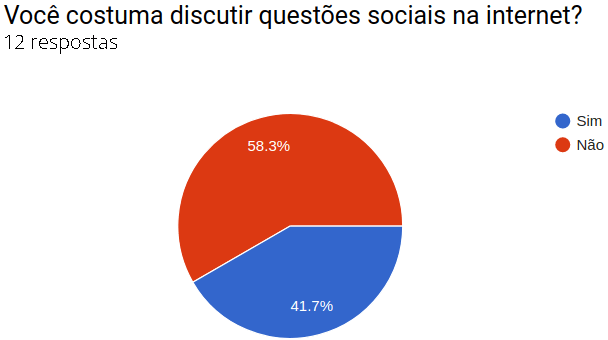
\includegraphics[scale=0.4]{./figuras/discutir.png}
    \caption{Participantes que discutem questões sociais na internet}
    \label{fig:grafico-discu}
\end{figure}

\begin{figure}[!ht]
    \centering
    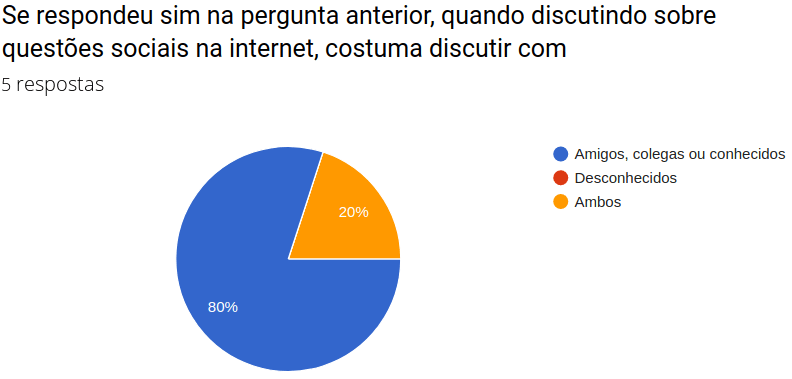
\includegraphics[scale=0.4]{./figuras/discutir_com.png}
    \caption{Grau de proximidade das pessoas que os participantes discutem questões sociais na internet.}
    \label{fig:grafico-discu-alvo}
\end{figure}
\pagebreak

\par
Quanto a última pergunta da primeira etapa, sobre o conhecimento do conceito de Taxonomia, percebeu-se que a grande maioria, 83,3\% não conhecia esse conceito conforme ilustra 
o gráfico na Figura \ref{fig:grafico-conhe-taxonomia}. Esse resultado pode ser um indicativo que mesmo a taxonomia sendo um modelo de classificação antigo e utilizado por diversas 
áreas do conhecimento, o conceito não faz parte do conjunto de conhecimento intrínseco das pessoas.

\begin{figure}[!ht]
    \centering
    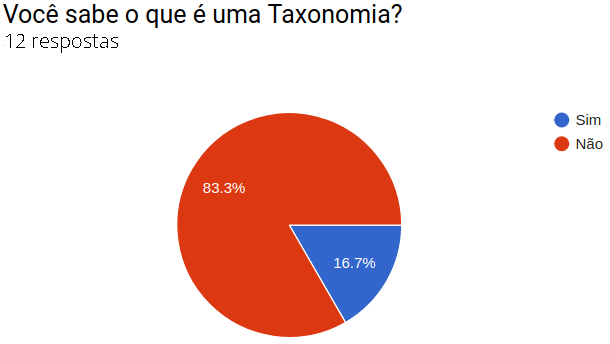
\includegraphics[scale=0.4]{./figuras/sabe_taxonomia.png}
    \caption{Conhecimento do conceito de taxonomia pelos participantes.}
    \label{fig:grafico-conhe-taxonomia}
\end{figure}

\par
O tempo médio dos participantes para a conclusão da classificação das duas ferramentas solicitadas foi de 24 minutos e 16 segundos. 
Notou-se que participantes com conhecimento prévio sobre ferramentas de participação realizaram 
as tarefas em um tempo 45\% menor se comparado ao restante da amostra, finalizando suas tarefas em 13 minutos e 17 segundos.

\par 
Outro ponto observado durante o experimento foi o fato de que, conforme os usuários fossem elaborando suas classificações,
essas informações foram utilizadas pelos próximos participantes, sinalizando a maneira colaborativa de evoluir a classificação das ferramentas.

A e-TAPE obteve um \textit{Score SUS} de 78,75, acima do valor de referência. A Tabela \ref{tab:resultado-questionario} apresenta a média de pontuação de cada item do questionário \acrshort{sus}.
Os gráficos com os resultados das respostas obtidas em cada  questão podem ser encontrado no Apêndice \ref{apendice:a}.

\begin{table}[!ht]
    \centering
    \caption{\textit{Score} de cada item do questionário aplicado}
    \label{tab:resultado-questionario}
    \begin{tabular}{l*{3}{>{\raggedright\arraybackslash}p{0.66\linewidth}p{0.1\linewidth}}}
    \toprule
    Nº & Questão & \textit{Score}    \\
    \midrule
    1 & Eu gostaria de utilizar este sistema sempre que fosse pesquisar sobre ferramentas de participação eletrônica. & 76,92 \\
    2 & Eu achei a aplicação desnecessariamente complexa. & 65,38 \\
    3 & Eu achei a aplicação fácil de usar. & 63,46 \\
    4 & Eu acho que precisaria de apoio de um suporte técnico para ser possível interagir com essa aplicação. & 61,54 \\
    5 & Eu achei que as diversas funções nesta aplicação foram bem integradas.  & 82,69 \\
    6 & Eu achei que houve muita inconsistência ou erros nesta aplicação.  & 86,54 \\
    7 & Eu imaginaria que a maioria das pessoas, interessadas em ferramentas de participação eletrônica, aprenderia a usar essa aplicação rapidamente. & 76,29 \\
    8 & Eu achei a aplicação muito complicada.  & 80,77 \\
    9 & Eu me senti muito confiante quanto às interações com essa aplicação.  & 59,62 \\
    10 & Eu precisei aprender muitas coisas sobre ferramentas de participação eletrônica para que eu pudesse fazer uso da aplicação. & 73,08 \\
    \bottomrule
    \end{tabular}
\end{table}

\par
Para realizar uma análise sobre os \textit{scores} obtidos pela e-TAPE, deve-se levar em consideração que, pela metodologia aplicada por \citeonline{brooke1996sus}, 
um valor próximo de 100 é uma avaliação favorável a aplicação. Sendo assim, o item melhor avaliado pelos participantes foi o item \textit{6 - Eu achei que houve muita inconsistência 
ou erros nesta aplicação.}, com uma média de 86,54, mostrando que, de fato, os participantes não encontraram muita inconsistência ou erros na aplicação.

Por outro lado, o item com o menor \textit{score}, foi o item \textit{9 - Eu me senti muito confiante quanto às interações com essa aplicação}, com valor de 59,62.
Levando em consideração o perfil dos participantes ( 91.70\%  não conhecem o conceito de participação eletrônica e 83,33\% não sabem o que é uma taxonomia), pode-se pensar que a falta conhecimento dos respondentes sobre os temas abordados na aplicação podem ter influenciado nessa reação. Dessa forma, é necessário criar estratégias que tornem esses conceitos mais familiares aos usuários como
vídeos e/ou tutoriais sobre o contexto participação eletrônica e a taxonomia.

\par
A Tabela \ref{tab:resultado-componentes} apresenta o resultado do questionário considerando os componentes de qualidade propostos
por \citeonline{nielsen199510}.

\begin{table}[!ht]
    \centering
    \caption{Valor dos componente de avaliação da qualidade da ferramenta e-TAPE}
    \label{tab:resultado-componentes}
    \begin{tabular}{l*{2}{>{\raggedright\arraybackslash}p{0.1\linewidth}}}
        \toprule
            Componente de Qualidade & Valor         \\
        \midrule
            Facilidade de aprendizagem & 68,75 \\
            Eficiência & 83,33 \\
            Facilidade de memorização & 65,38 \\
            Minimização dos erros & 86,54 \\
            Satisfação & 66,02\\
        \bottomrule
        \end{tabular}
\end{table}

O preceito válido para os itens em individual pode ser também aplicado aos componentes de qualidade do \textit{software}, ou seja, quanto mais próximo ao valor 100, melhor é o resultado do componente.
Após análise dos valores, conclui-se:
\begin{itemize}
    \item \textbf{Facilidade de aprendizagem}: representada pelos itens 3, 4, 7 e 10. A média obtida foi 68,75, valor 0.75 acima do valor de referência. Esse resultado indica que, mesmo a aplicação e-TAPE encontrando-se em um estágio inicial, foi considerada apta para ser utilizada. Por outro lado, o fato da média obtida ser muito próxima do valor de referência é um indicativo da necessidade de facilitar o aprendizado das funcionalidades. 

    \item \textbf{Eficiência}: representada pelos itens 5, 6 e 8. A média obtida foi 83,33. Esse resultado indica que depois de saber usar a ferramenta, o usuário consegue aumentar sua produtividade fazendo com que sua interação seja mais eficiente. Essa conclusão pode ser corroborada pelo valor obtido pelo componente minimização de erros.

    \item \textbf{Facilidade de memorização}: representada pelo item 2, obteve média de 65,38, valor 2,62 abaixo do valor de referência. Esse resultado reforça o a problemática discutida anteriormente, a necessidade de uma área na aplicação, na qual o usuário possa aprender mais sobre os conceitos abordados e também sobre 
          a aplicação. O valor obtido por esse componente evidencia a necessidade de disponibilizar recursos que ampliem as possibilidades de ajuda ao usuário.

    \item \textbf{Minimização dos erros}: representada pelo item 6, a média obtida foi 86,54, item com a melhor avaliação. Se correlacionado com o valor do componente eficiência, mostra que a aplicação conseguiu gerar uma resposta positiva aos participantes em componentes considerados importantes que são a eficiência e a quantidade de erros. 

    \item \textbf{Satisfação}: representado pela média das questões 1, 4 e 9, o valor obtido foi 66,02. O fato da satisfação ter sido abaixo do valor de referência pode ser justificado tanto pela falta de conhecimento dos usuários sobre os temas abordados, ponto já discutido, quanto pela dificuldade de aprendizado da interface (componente facilidade de aprendizado) e reforça ainda mais a necessidade de melhorias quanto à experiência do usuário. 
         
\end{itemize}


Ao final do questionário, foi disponibilizado um espaço, de preenchimento opcional para  inserção de comentários sobre a aplicação. Ao total, 
4 comentários foram deixados pelos participantes e estão descritos na Tabela \ref{tab:coments}.

\pagebreak
\begin{table}[!ht]
    \centering
    \caption{Comentários dos participantes}
    \label{tab:coments}
    \begin{tabular}{l*{2}{>{\raggedright\arraybackslash}p{0.70\linewidth}}}
    \toprule
        Nº & Comentário        \\
    \midrule
        1 & Acho que no momento de responder sobre a aplicação a ajuda do mapa poderia trazer mais exemplos em algumas opções. \\
    \midrule
        2 & Acredito que o uso não é complicado mas requer certa prática, portanto uma interface mais auto-explicativa ajudaria. \\
    \midrule
        3 & Na minha opinião, o sistema é promissor, promove uma boa interação e bom uso dos aplicativos e plataformas eletrônicas para uso do dia a dia. Entretanto, o entendimento da funcionalidade da ferramenta aumentou gradualmente com o conhecimento dos conceitos e da aplicabilidade, através de exemplos. Talvez a aplicação do exemplo em texto do Colab e Triang dentro das árvores, tornaria esse entendimento mais rápido. Porém, acredito na existência de pelo menos dois tipos de usuários desses aplicativos. O primeiro tipo é um usuário com curiosidade e fome por conhecimento técnico da ferramenta, este irá procurar entender os conceitos da taxonomia além de apenas contribuir com a aplicação. O outro tipo de usuário não possui conhecimento ou fome pela raíz técnica da ferramenta, e prefere menos informações durante o uso. Assim, uma boa forma de garantir a usabilidade de ambos os supostos usuários descritos, é que a plataforma tenha opção para uma interface com informações completas a respeito do funcionamento da ferramenta (uma opção "desenvolvedor" por exemplo), e uma opção "simple" onde o segundo tipo de usuário se sentirá confortável em contribuir com a ferramenta. \\
    \midrule
        4 & Layout é atrativo e a ferramenta é amigável. Além disso, as explicações são objetivas e de fácil compreensão. \\
    \bottomrule
    \end{tabular}
\end{table}

\par
Observa-se pelos comentários, características que foram retratadas pelos componentes de qualidade de software, apresentados na Tabela \ref{tab:resultado-componentes}.
Mais especificamente, o terceiro comentário sugere a inclusão de requisito funcional para a criação de dois modos de interação com a e-TAPE, alternando entre um
modo para especialistas e outro para leigos sobre o assunto.

\par 
Diante dos resultados apresentados, pode-se afirmar que a aplicação e-TAPE, embora tenha apresentado um comprometimento em alguns atributos de qualidade, 
conseguiu uma boa avaliação de usabilidade. Os problemas identificados serão traduzidos em requisitos funcionais para as próximas versões da ferramenta. 
O capítulo \ref{cap:cap5} retrata o futuro da aplicação.  
